% !TEX TS-program = pdflatex
% !TEX encoding = UTF-8 Unicode

% This is a simple template for a LaTeX document using the "article" class.
% See "book", "report", "letter" for other types of document.

\documentclass[11pt]{article} % use larger type; default would be 10pt

\usepackage[utf8]{inputenc} % set input encoding (not needed with XeLaTeX)

%%% Examples of Article customizations
% These packages are optional, depending whether you want the features they provide.
% See the LaTeX Companion or other references for full information.

%%% PAGE DIMENSIONS
\usepackage{geometry} % to change the page dimensions
\geometry{a4paper} % or letterpaper (US) or a5paper or....
\geometry{margin=1in} % for example, change the margins to 2 inches all round
% \geometry{landscape} % set up the page for landscape
%   read geometry.pdf for detailed page layout information

% \usepackage[parfill]{parskip} % Activate to begin paragraphs with an empty line rather than an indent

%%% PACKAGES
\usepackage{booktabs} % for much better looking tables
\usepackage{array} % for better arrays (eg matrices) in maths
\usepackage{paralist} % very flexible & customisable lists (eg. enumerate/itemize, etc.)
\usepackage{verbatim} % adds environment for commenting out blocks of text & for better verbatim
\usepackage{subfig} % make it possible to include more than one captioned figure/table in a single float
\usepackage{authblk} % allows for multiple authors and affiliations
\usepackage{amsmath} % for \text{} command
\usepackage{makecell, siunitx} % allows table headers to be two lines
\usepackage{graphicx} % support the \includegraphics command and options
\graphicspath{ {images/} } % image file path
\usepackage{verbatim} % for comments
\linespread{1.3} % changes line spacing to 1.5 line spacing
\usepackage{mhchem} % for typesetting chemical formulae
\usepackage{float} % for positioning floats

\usepackage{titlesec} % for changing section font sizes
\begin{comment}
\titleformat*{\section}{\large\bfseries}
\titleformat*{\subsection}{\normalsize\bfseries}
\titleformat*{\subsubsection}{\large\bfseries}
\titleformat*{\paragraph}{\large\bfseries}
\titleformat*{\subparagraph}{\large\bfseries}
\end{comment}

% These packages are all incorporated in the memoir class to one degree or another...

%%% HEADERS & FOOTERS
\usepackage{fancyhdr} % This should be set AFTER setting up the page geometry
\pagestyle{fancy} % options: empty , plain , fancy
\renewcommand{\headrulewidth}{0pt} % customise the layout...
\lhead{}\chead{}\rhead{}
\lfoot{}\cfoot{\thepage}\rfoot{}

%%% SECTION TITLE APPEARANCE
%\usepackage{sectsty}
%\allsectionsfont{\sffamily\mdseries\upshape} % (See the fntguide.pdf for font help)
% (This matches ConTeXt defaults)

%%% ToC (table of contents) APPEARANCE
\usepackage[nottoc,notlof,notlot]{tocbibind} % Put the bibliography in the ToC
\usepackage[titles,subfigure]{tocloft} % Alter the style of the Table of Contents
\renewcommand{\cftsecfont}{\rmfamily\mdseries\upshape}
\renewcommand{\cftsecpagefont}{\rmfamily\mdseries\upshape} % No bold!

%%% END Article customizations

%%% The "real" document content comes below...

\title{Synthesizing and and Measuring the Efficacy of Zeolites}
\author[*]{Hunter Ducharme}
\author[ ]{Brianna Hill}
\affil[*]{Primary author}
\date{} % Activate to display a given date or no date (if empty),
         % otherwise the current date is printed 

\begin{document}
\maketitle

\begin{abstract}
Polycyclic aromatic hydrocarbon (PAH) is a very common type of pollutant found in the environment. It is speculated that these pollutants can be removed by having them be absorbed into a porous material such as coal, zeolite, or magnetized zeolite. This experiment tested the absorptivity of each precipitant on a solution of procion red. It was found that magnetized zeolites absorbed the most amount of red dye solution, suggesting they might be a good material for removing PAHs from the enviornment.
\end{abstract}

\section{Introduction}
The production of materials by plants and factories has resulted in the constant release of harmful pollutants which leads to the need for a method that can withdraw these toxins from the environment. One group of pollutants of interest are polycyclic aromatic hydrocarbons (PAHs), because they are speculated to be carcongenic to humans and aquatic wildlife \cite{PAH}. They are commonly found in cold-tar and asphalt sealants, in addition to industrial and municipal wastewater \cite{Southworth1979}. It is commonly thought that using porous materials would be a viable way to combat this problem in water environments through their ability to absorb chemicals. This paper attemps to test the efficacy of magnetic zeolites in absorbing a red dye solution in hopes of applying this method to the removal of PAHs in water sources.

\section{Materials and Methods}

\subsection{Synthesizing the Zeolites}
First, sodium hydroxide (3.0M \ce{NaOH}, 50 mL) and sodium aluminate (\ce{NaAlO2}$\cdot${5H2O}; 3.7558 g) were added to a beaker which was then placed on a hotplate/stirrer (190$^{\circ}$ C; 240 rpm). Simeltaneously, distilled water (50 mL) was brought to a boil. Sodium silicate (\ce{Na2SiO3}$\cdot$\ce{5H2O}; 2.6523 g) was added to the boiling water and stirred. Once both solutions were at a gentle boil, the sodium silicate solution was added to the sodium aluminate solution and held at 90$^{\circ}$ for 60 minutes while stirring. Lastly, the entire soultion was split between two centrifuge tubes (\large 15 mL each) and placed in a centrifuge for 10 minutes at 5000 rpm.

\subsection{Synthesizing the Magnetized Zeolites}
Reference section 2.1. Synthesizing magnetized zeolites shares the same process as synthesizing regular zeolites, however, after holding the solution for 60 minutes, \ce{FeCl3} (0.78 g) and \ce{FeSO4}$\cdot$\ce{7H2O} (0.39 g) were then added until fully dissolved. Lastly, the same centrifuge step was applied and this solution was placed in a centrifuge for 10 minutes at 5000 rpm.

\subsection{Preparing Samples for Spectrometer}
First, a beaker was filled (\large 100 mL) with a red dye stock solution (.05mM; \large procion red). Three centrifuge tubes were then filled (\large 15ml each) with the red dye stock solution and either contained regular zeolite (.1021 g), magnetized zeolite (.1009 g), or coal (.1032 g; which was grinded with a mortar and pestle). The tubes were then placed in a centrifuge for 10 minutes at 2000 rpm. While the tubes were in the centrifuge, three serial dilutions of the stock solution (50\%, 25\%, and 12.5\%) were made using a 5 mL pipet and a 10 mL volumetric flask. The samples containing the precipitants were allowed to sit for 5 minutes and soak up the red dye. Lastly, each precipitant solution was filtered into a cuvette for use in the spectrometer.

\subsection{Data Collection}
All solutions were placed inside of cuvettes in preparation for use with a spectrometer. A spectrometer was connected to a computer and calibrated with distilled water using the software Logger \textit{Pro}. After calibrating the device, the stock solution was placed in the spectrometer and spectra data was collected to find $\lambda_{max}$. Lastly, the absorption for each sample was then collected at $\lambda_{max}$.
\begin{comment}
Using the .cmbl file containing the three different spectra, a graph was produced containing the absorbance vs. wavelength plots for each sample. The maximum wavelength $\lambda_{\text{max}}$ was recorded from the graphs for bromothymol blue (HBB) and bromothymol blue anion ($\text{BB}^-$). For each $\lambda_{\text{max}}$ found, the absorption of each solution was recorded using the data table in the left-hand pane of Logger \textit{pro}. Any existing isobestic points were found and recorded using the same procedure as the last step. Lastly, the absorption for each sample was found at the wavelength 616 nm using the data table in the left-hand pane of Logger \textit{Pro}. 
\end{comment}

\section{Results and Discussion}

\subsection{Data Summary}
For section 2.4, it was found that $\lambda_{max}$ was 535.5 nm for the red dye. This value corresponds with the wavelength where the absorption of the dye is at its maximum. According to Beer's Law, $A = \varepsilon b c$, where $A$ is absorbance, $b$ is the path length (cm), $\varepsilon$ is the molar absorptivity (mM$^{-1} \cdot$cm$^{-1}$), and $c$ is the concentration (mM). To find the concentrations of the precipitant solutions, a calibration curve was first made using the concentration and absorption data of the diluted samples to get an equation that represents the graph. The equation of the best-fit line was found to be $y = 13.286x$, which is Beer's Law $A = \varepsilon b c$. 

\begin{figure}[H]
    \centering
    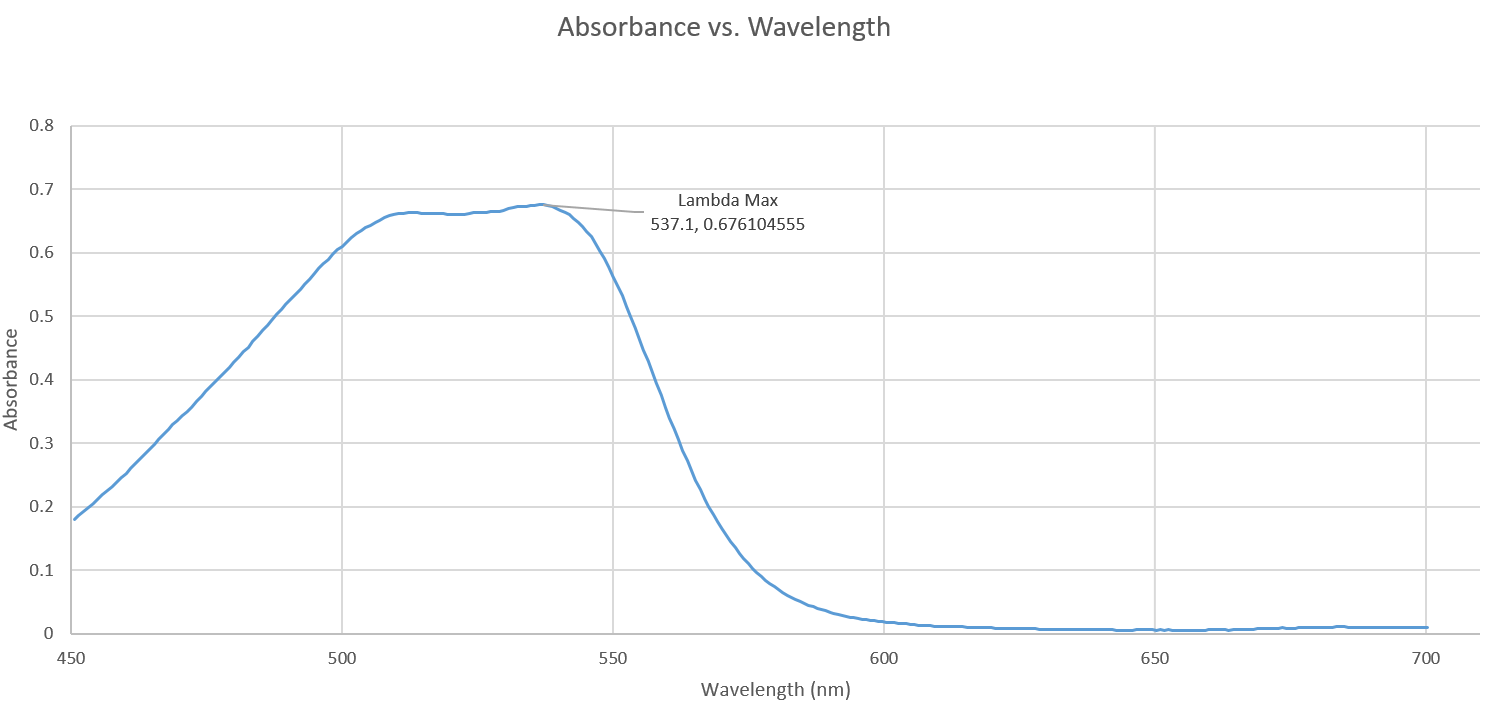
\includegraphics[width=\linewidth]{spectra_graph}
    \caption{The absorbance vs. wavelength plot for the undiluted sample of procion red.}
    \label{fig:mesh1}
\end{figure}

\begin{align*}
A = \varepsilon bc \\
c = \frac{A}{b\cdot \varepsilon} \\
c_{\text{coal solution}} = \frac{0.335}{13.286} \approx .025215 \ \text{mM} \\
c_{\text{zeolite solution}} = \frac{0.382}{13.286} \approx .028752 \ \text{mM}\\
c_{\text{mag zeolite solution}} = \frac{0.312}{13.286} \approx .002348 \ \text{mM}
\end{align*}
\\
Table 1.1 summarizes the absorption for each sample at $\lambda_{max}$ and the remaining concentrations of the preciptant solutions. The 'Corrected Absorbance' column is the difference between the sample's absorption at 535 nm and its absorption at 750 nm.

\begin{table}[H]
\resizebox{\textwidth}{!}{%
\centering
\begin{tabular}{ccccc}
\thead{Sample}               & \thead{Concentration (mM)} & \thead{Absorption (535.5 nm)} & \thead{Absorption (750 nm)} & \thead{Corrected Absorbance} \\
100\% .05mM Red Dye  & .05                & .666241               &         -            &       -                \\
50\% .05mM Red Dye   & .025               & .323556               &             -        &         -              \\
25\% .05mM Red Dye   & .0125              & .166226               &              -       &       -                \\
12.5\% .05mM Red Dye & .00625           & .101474               &               -      &       -                \\
Charcoal Solution            &     .025215                  & .400                  & .065                & .335                  \\
Zeolite Solution            &         .028752             & .440                  & .058                & .382                  \\
Magnetized Zeolite Solution  &       .002348                & .368                  & .056                & .312                 
\end{tabular}}
\caption{The concentration of each solution and its absorbance at $\lambda_{\text{max}}$.}
\end{table}

Therefore, based on Table 1.1, the magnetized zeolite solution has the lowest corrected absorbance which refers to being more efficient at absorbing the red dye stock solution. These results suggest that magnetized zeolite is superior to charcoal and regular zeolite in absorbing procion red.

\subsection{Discussion}
There are a few parameters that can be used to compare the usefulness of charcoal to zeolites. One parameter is the method used in this experiment-absorptivity. A second parameter is the magnetic properties of each precipitant. The magnetic property of the material could effect the ability to absorb PAHs. Lastly, another parameter that could be of importance when choosing a material is the availability and cost of each. When deciding one material over the other, a few things the EPA should consider is the biodegradable property of each material, whether or not they give off harmful by-products, and their effects on the animals and ecosystem in which they were being placed.

The structure of procion red and Benzo(a)pyrene are similar to an extent. The structures are close enough for procion red to act as a suitable model for PAHs. Procion red is a fairly flat molecule and can be absorbed through intercalation.

A few possible sources of errors include (a) not making sure the cuvettes were entirely clean before placing them in the spectrometer, (b) one filter paper filtering a solution better than another filter paper, (c) not cleaning the lens on the spectrometer where the light is shot out of, and (e) having contaminates inside of the solutions such as small dirt particles or other things that would hinder the passage of light through the solution.

\section{Conclusion}
This experiment was performed to compare the usefulness of coal, zeolites, and magnetized zeolites in absorping a red dye solution with hopes of applying this to absorbing harmful PAHs in the environment. It was found that magnetized zeolites absorbed more red dye than did coal and regular zeolites. This experiment successfully determined which precipitant is the most useful in absorbing procion red, and potentially the most useful in absorbing PAHs.


\newpage 
\bibliography{research_project} 
\bibliographystyle{apalike}


\end{document}